\sectionthree{The Prime Number Theorem and finding primes}
\begin{python0}
from solutions import *; clear()
\end{python0}

We'll need a way to create huge primes for RSA.

Of course you know Euclid's theorem that says
there are infinitely many primes.
So we don't have to worry about not finding them.
But just because there are infinitely many primes, it does not mean
they are everywhere!

Generally, we want to specify how large our primes should be.
This is specified by the bit length of the primes.
Given the length, one can generate a sequence of bits of that length.
Of course that number should be odd.
So the least significant bit is set to $1$.
Call this $n$.
One can than check if $n$ is a prime.
If $n$ is not prime, we try $n + 2$, etc.

Does this process take a long time?

Gauss was the first to realize that even though primes seem to appear
randomly on the real line,
\begin{center}
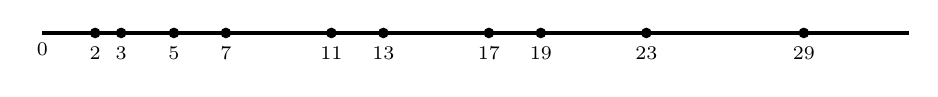
\begin{tikzpicture}
\draw[line width=0.04cm,black] (0,0) to  (11.0,0);

\fill[black] (0.67, 0.0) circle (0.06);
\draw[black] (0.67, 0.0) circle (0.06);
\node[anchor=north] at (0.67,-0.06)   {{\scriptsize $2$}};

\fill[black] (1.0, 0.0) circle (0.06);
\draw[black] (1.0, 0.0) circle (0.06);
\node[anchor=north] at (1.0,-0.06)   {{\scriptsize $3$}};

\fill[black] (1.67, 0.0) circle (0.06);
\draw[black] (1.67, 0.0) circle (0.06);
\node[anchor=north] at (1.67,-0.06)   {{\scriptsize $5$}};

\fill[black] (2.33, 0.0) circle (0.06);
\draw[black] (2.33, 0.0) circle (0.06);
\node[anchor=north] at (2.33,-0.06)   {{\scriptsize $7$}};

\fill[black] (3.67, 0.0) circle (0.06);
\draw[black] (3.67, 0.0) circle (0.06);
\node[anchor=north] at (3.67,-0.06)   {{\scriptsize $11$}};

\fill[black] (4.33, 0.0) circle (0.06);
\draw[black] (4.33, 0.0) circle (0.06);
\node[anchor=north] at (4.33,-0.06)   {{\scriptsize $13$}};

\fill[black] (5.67, 0.0) circle (0.06);
\draw[black] (5.67, 0.0) circle (0.06);
\node[anchor=north] at (5.67,-0.06)   {{\scriptsize $17$}};

\fill[black] (6.33, 0.0) circle (0.06);
\draw[black] (6.33, 0.0) circle (0.06);
\node[anchor=north] at (6.33,-0.06)   {{\scriptsize $19$}};

\fill[black] (7.67, 0.0) circle (0.06);
\draw[black] (7.67, 0.0) circle (0.06);
\node[anchor=north] at (7.67,-0.06)   {{\scriptsize $23$}};

\fill[black] (9.67, 0.0) circle (0.06);
\draw[black] (9.67, 0.0) circle (0.06);
\node[anchor=north] at (9.67,-0.06)   {{\scriptsize $29$}};

\node[anchor=north] at (0,0)   {{\scriptsize $0$}};
\end{tikzpicture}

\end{center}


the density of primes seems to follow some
law.
The density of primes can be defined this way.
Let $\pi(x)$ be the number of primes $\leq x$.
Then the density of primes up to $x$ is
\[
\frac{\pi(x)}{x}
\]
Here is the plot of $\pi(x)$ up to $x = 20$:
\input{pi_x_20.tex}
When the plot is up to $x = 100$ one begin to see that the
rough and jagged graph begin to smooth out:
\input{pi_x_100.tex}

Through analyzing tables of primes, Gauss discovered that
$\pi(x)/x$ is \defone{asymptotically equivalent} to $1/\ln x$ ($\ln = \log_e$)
\[
\frac{\pi(x)}{x} \sim \frac{1}{\ln x}
\]
i.e.,
\[
\lim_{x \rightarrow \infty} \frac{\pi(x)/x}{1/\ln x} = 1
\]
Equivalently
\[
\pi(x) \sim \frac{x}{\ln x}
\]
Here a plot of $\pi(x)$ and $x/\ln x$ up to $x = 10^5$:
[OMITTED]
%\input{pi_x_100000.tex} $ <<<<<<< tex memory liit exceeded

The above was first conjectured by Gauss in 1792/3
and finally proven in 1896 by
\href{https://en.wikipedia.org/wiki/Jacques_Hadamard}{Hadamard}
and
\href{https://en.wikipedia.org/wiki/Charles_Jean_de_la_Vall%C3%A9e_Poussin}{de la Vallée Poussin}:

\begin{thm} \textnormal{(\defone{Prime Number Theorem})}
\[
\pi(x) \sim \frac{x}{\ln x}
\]  
\end{thm}

Among number theorists and researchers in cryptography,
the above deep result is known as \defone{PNT}.

By PNT, when $x$ is large, the density of primes up to $x$ is approximately
$1/\ln x$.
Using the sieve of Eratosthenes, the number of primes up to $x = 10^5$ is
$9592$, i.e., $\pi(x)/x = 9592/100000 = 0.09592 = 9.592\%$
which is very close to $1/\ln x = 1/\ln 10^5 = 0.086858... = 8.6858...\%$.
If we search for a prime only among \textit{odd} integers, the
chance of finding a prime is $2/\ln x = 0.173717... = 17.3717...\%$.

For modern-day RSA, primes used have approximately 1024-2048 bits.
If we choose a bit length of 1024, then
$2/\ln 2^{1024} = 0.1408...\%$.
Therefore one might find a prime after $< 1000$ tries among odd integers.
Usually one would begin with an integer $n$
with a random sequence of 1024 bits, with least
significant bit being 1 (so that $n$ is odd).
Then a primality test is used to check if $n$ is prime.
We'll see that a probabilistic primality test is used.
If $n$ is not a prime, one would then try $n + 2$. Etc.

Next we will look at two very important primality tests: Fermat primality test
and Miller--Rabin primality test.
Miller--Rabin primality test is the one that is used in the real world.
However the main idea in Miller--Rabin primality test is
actually Fermat primality test.


\begin{ex} 
  \label{ex:rsa-10}
  \tinysidebar{\debug{exercises/{nt-61/question.tex}}}
  In your \verb!Zmod.py!, complete the following methods:
  \begin{enumerate}[nosep]
    \li multiplicative inverse mod $N$ (i.e., \texttt{inv})
    \li invertibility mod $N$ (i.e., \texttt{is\_invertible})
    \li division (i.e., \texttt{\_\_div\_\_})
  \end{enumerate}

  \solutionlink{sol:rsa-10}
  \qed
\end{ex} 
\begin{python0}
from solutions import *
add(label="ex:rsa-10",
    srcfilename='exercises/rsa-10/answer.tex') 
\end{python0}


\begin{ex} 
  \label{ex:rsa-10}
  \tinysidebar{\debug{exercises/{nt-61/question.tex}}}
  In your \verb!Zmod.py!, complete the following methods:
  \begin{enumerate}[nosep]
    \li multiplicative inverse mod $N$ (i.e., \texttt{inv})
    \li invertibility mod $N$ (i.e., \texttt{is\_invertible})
    \li division (i.e., \texttt{\_\_div\_\_})
  \end{enumerate}

  \solutionlink{sol:rsa-10}
  \qed
\end{ex} 
\begin{python0}
from solutions import *
add(label="ex:rsa-10",
    srcfilename='exercises/rsa-10/answer.tex') 
\end{python0}


\begin{ex} 
  \label{ex:rsa-10}
  \tinysidebar{\debug{exercises/{nt-61/question.tex}}}
  In your \verb!Zmod.py!, complete the following methods:
  \begin{enumerate}[nosep]
    \li multiplicative inverse mod $N$ (i.e., \texttt{inv})
    \li invertibility mod $N$ (i.e., \texttt{is\_invertible})
    \li division (i.e., \texttt{\_\_div\_\_})
  \end{enumerate}

  \solutionlink{sol:rsa-10}
  \qed
\end{ex} 
\begin{python0}
from solutions import *
add(label="ex:rsa-10",
    srcfilename='exercises/rsa-10/answer.tex') 
\end{python0}


\begin{ex} 
  \label{ex:rsa-10}
  \tinysidebar{\debug{exercises/{nt-61/question.tex}}}
  In your \verb!Zmod.py!, complete the following methods:
  \begin{enumerate}[nosep]
    \li multiplicative inverse mod $N$ (i.e., \texttt{inv})
    \li invertibility mod $N$ (i.e., \texttt{is\_invertible})
    \li division (i.e., \texttt{\_\_div\_\_})
  \end{enumerate}

  \solutionlink{sol:rsa-10}
  \qed
\end{ex} 
\begin{python0}
from solutions import *
add(label="ex:rsa-10",
    srcfilename='exercises/rsa-10/answer.tex') 
\end{python0}


\begin{ex} 
  \label{ex:rsa-10}
  \tinysidebar{\debug{exercises/{nt-61/question.tex}}}
  In your \verb!Zmod.py!, complete the following methods:
  \begin{enumerate}[nosep]
    \li multiplicative inverse mod $N$ (i.e., \texttt{inv})
    \li invertibility mod $N$ (i.e., \texttt{is\_invertible})
    \li division (i.e., \texttt{\_\_div\_\_})
  \end{enumerate}

  \solutionlink{sol:rsa-10}
  \qed
\end{ex} 
\begin{python0}
from solutions import *
add(label="ex:rsa-10",
    srcfilename='exercises/rsa-10/answer.tex') 
\end{python0}

